\chapter{Tumblr Data}

%%%%%%%%%%%%%%%%%%%%%%%%%%%%%%%%%%%%%%%%%%%%%%%%%%%%%%%%%%%%
%%%%%%%%%%%%%%%%%%%%  NEW SECTION   %%%%%%%%%%%%%%%%%%%%%%%%
%%%%%%%%%%%%%%%%%%%%%%%%%%%%%%%%%%%%%%%%%%%%%%%%%%%%%%%%%%%%
\section{Overview of the Data}
Tumblr posts were retrieved using the Python API, here is an example of a post:
\begin{figure}[H]
\centering

\includegraphics[width=.58\textwidth]{Images/chowchow.png}
\caption{An example of a Tumblr post}
\end{figure}

The tags `\#chowchow \# home \#happy \#bluetongue' are really valuable as they indicate the user's state of mind when writing that post. Ekman popularised the idea that there are six basic emotions \cite{ekman}: hapiness, sadness, anger, surprise, fear, disgust. These emotions are said to be {\em basic} as they are hardwired regardless of the species: basic emotions are innate, universal and automatic and induce fast reactions that are linked with a high survival rate.

To build our dataset, queries were made searching for each of the six emotions appearing in the tags. Adjectives were used as they were more commonly used by users: \#happy, \#sad, \#angry, \#surprised, \#scared and \#disgusted. Each post would then contain the following information:
\begin{enumerate}
\item The text. In the example above: \textit{When dogs are back home!}
\item The image.
\item The associated emotion: one among the six classes.
\end{enumerate}

Note that sometimes, a post would contain several basic emotions such as `\#sad \#angry'. We simply selected the first hashtag written by the user as it can be deemed as the main emotion that the user first thought of.

The data extraction took several weeks due to the API's limitations: 1,000 requests per hour and 5,000 requests per day, with each request containing 20 posts. The dataset contains about 1 million posts.

\section{Data Preprocessing}
In some posts, the tag also appeared in the text itself, for instance:
\begin{quote}
\textit{``When you're on vacations and there is a rainstorm. \#fail \#sad"}.
\end{quote}
Keeping the \textit{\#sad} would bias the learning process and the neural network would simply learn to detect the presence or absence of that tag. To ensure that the network is actually learning something, we removed from the text the hashtags containing the emotion to be predicted.

Also, Tumblr is used worldwide, therefore posts not written in English had to be removed from the training data. Basically, if a post contains less than a given number of English word, it is deemed as non-English and removed from the dataset. The threshold was set to 5 English words as it appears to filter out reasonably well the dataset. The vocabulary of English words was obtained from Word2Vec and will be detailed further in Section 4.

Figure \ref{fig:emotions} shows examples of posts with their associated emotions:

\begin{figure}
\begin{subfigure}[t]{.5\textwidth}
  \vskip 0pt %Necessary to align on image and not caption
  \centering
  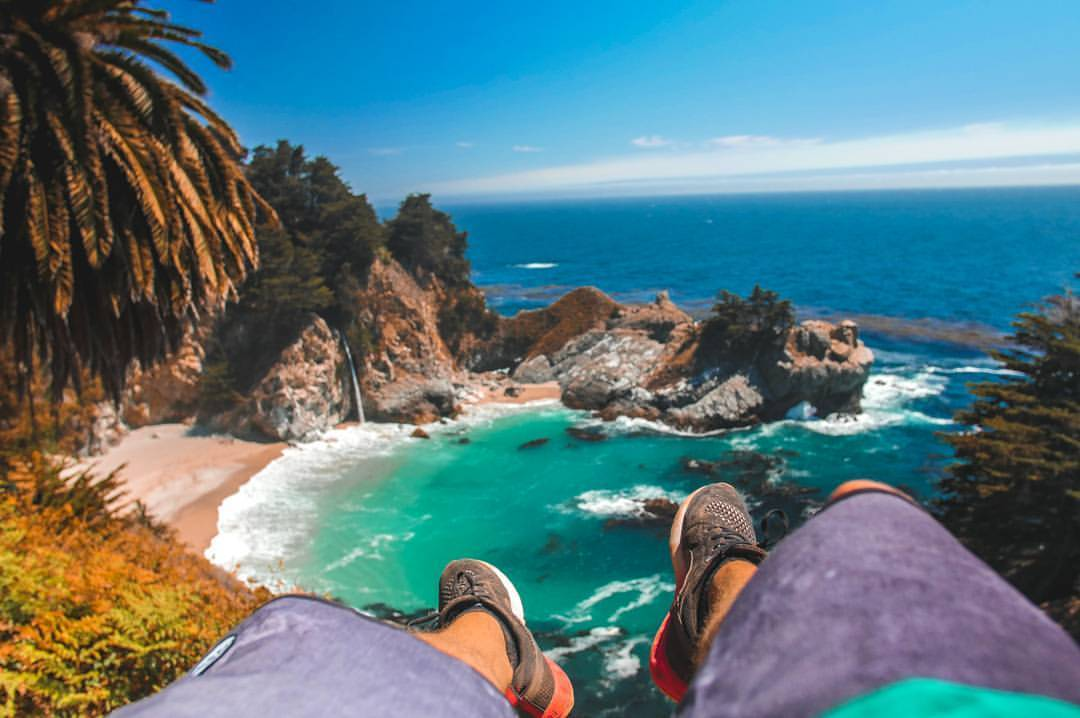
\includegraphics[width=.8\linewidth]{Images/happy.jpg}
  \caption{\textbf{Happy}: ``Just relax with this amazing view \#bigsur \#california \#roadtrip \#usa \#life \#fitness (at McWay Falls)"}
\end{subfigure}
\begin{subfigure}[t]{.5\textwidth}
  \vskip 0pt 
  \centering
  
\includegraphics[width=.7\linewidth]{Images/scared.jpg}
  \caption{\textbf{Scared}: ``On a plane guys! We're about to head out into the sky to Paris, France \#Paris \#trip \#kinda \#nervous \#fun \#vacations"}
\end{subfigure}
\begin{subfigure}[t]{.5\textwidth}
  \vskip 0pt
  \centering
  
\includegraphics[width=.6\linewidth]{Images/sad.jpg}
  \caption{\textbf{Sad}: ``It's okay to be upset. It's okay to not always be happy. It's okay to cry. Never hide your emotions in fear of upsetting others or of being a bother   If you think no one will listen. Then I will."}
\end{subfigure}
\begin{subfigure}[t]{.5\textwidth}
  \vskip 0pt 
  \centering
  
\includegraphics[width=.5\linewidth]{Images/angry.jpg}
  \caption{\textbf{Angry}: ``Tensions were high this Caturday..."}
\end{subfigure}
\begin{subfigure}[t]{.5\textwidth}
  \vskip 0pt 
  \centering
  
\includegraphics[width=.8\linewidth]{Images/surprised.jpg}
  \caption{\textbf{Surprised}: ``Which Tea? Peppermint tea: What is your favorite gif right now?"}
\end{subfigure}
\begin{subfigure}[t]{.5\textwidth}
  \vskip 0pt 
  \centering
  
\includegraphics[width=.8\linewidth]{Images/disgusted.jpg}
  \caption{\textbf{Disgusted}: ``Me when I see a couple expressing their affection in physical ways in public"}
\end{subfigure}
\caption{The 6 emotions illustrated by Tumblr posts \cite{tumblr-photos}}
\label{fig:emotions}
\end{figure}